% Corrigé — Torseur de cohésion des portiques plans isostatiques — Structure (S4)
% Compilation : xelatex corrige-s4.tex (deux passes, pour la pagination « n / N »)
% =====================================================================
%  Préambule commun aux corrigés « MS – Mécanique des Structures 3 »
%  Reproduit la charte du corrigé de référence Structure (S6) v2 :
%  A4, cadre, en-tête « Science / MS – Mécanique des Structures 3 » + logo,
%  pied « MS – TD / titre » + pagination « n / N ».
% =====================================================================
\documentclass[10pt,a4paper]{article}

\usepackage[a4paper,
  left=48.8bp, textwidth=511.7bp,
  top=42.4bp, textheight=738bp,
  headheight=0pt, headsep=0pt, footskip=0pt]{geometry}

\usepackage{fontspec}
\usepackage{unicode-math}
\setmainfont{Liberation Serif}[Ligatures=TeXOff]
\newfontfamily\carlito{Carlito}
\newfontfamily\caladea{Caladea}
\setmathfont{Latin Modern Math}
\setmathfont{Caladea Italic}[range={it/{latin,Latin}->up}]
\setmathfont{Caladea}[range={up/{num}}]

\usepackage[french]{babel}
\usepackage{xcolor}
\usepackage{graphicx}
\usepackage{array}
\usepackage{colortbl}
\usepackage{eso-pic}
\usepackage{lastpage}
\usepackage{tikz}
\usetikzlibrary{arrows.meta,calc,patterns.meta,shadings}

\graphicspath{{img/}}
\linespread{0.958}
\setlength{\parindent}{0pt}
\setlength{\parskip}{2.6pt}
\pagestyle{empty}
\raggedbottom
\frenchsetup{SmallCapsFigTabCaptions=false}

% ------------------------------------------------------------------ couleurs
\definecolor{titreBleu}{RGB}{23,54,93}
\definecolor{filetBleu}{RGB}{79,129,189}
\definecolor{secBleu}{RGB}{54,95,145}
\definecolor{bandeBleu}{RGB}{219,229,241}
\definecolor{bleuConnu}{RGB}{31,73,125}
\definecolor{rougeInc}{RGB}{192,0,0}
\definecolor{aplat}{RGB}{185,205,229}
\definecolor{noirBarre}{RGB}{17,17,17}
\definecolor{grisRes}{RGB}{128,128,128}
\definecolor{grisCote}{RGB}{168,168,168}

% ------------------------------------------------------------------ maths
% Espacement aéré des équations centrées, comme sur le corrigé de référence
\everydisplay\expandafter{\the\everydisplay\thickmuskip=12mu plus 4mu\medmuskip=7mu plus 2mu}
\newcommand{\dMdx}{\frac{\mathrm{d}M}{\mathrm{d}x}}
\newcommand{\ok}{\;\checkmark}
\newcommand{\Sq}{(S\textsubscript{4})}

% ------------------------------------------------------------------ en-tête, pied, cadre
\newcommand{\TitreCourt}{Torseur de cohésion des portiques plans isostatiques}
\AddToShipoutPictureBG{%
  \begin{tikzpicture}[remember picture,overlay,x=1bp,y=1bp]
    \coordinate (O) at (current page.south west);
    % en-tête
    \node[anchor=base west,inner sep=0pt,font=\fontsize{6}{7}\selectfont] at ($(O)+(43,815.55)$) {Science};
    \node[anchor=base west,inner sep=0pt,font=\fontsize{6}{7}\selectfont] at ($(O)+(43,807.85)$) {MS – Mécanique des Structures 3};
    \node[anchor=north west,inner sep=0pt] at ($(O)+(512.65,827.7)$) {
\includegraphics[width=52.9bp,height=28bp]{logo-gc.png}};
    % cadre (tracé après le logo pour rester visible)
    \draw[line width=0.5bp] ($(O)+(38,54.89)$) rectangle ($(O)+(571,802.89)$);
    % pied de page
    \node[anchor=base west,inner sep=0pt,font=\fontsize{6}{7}\selectfont] at ($(O)+(43,31.15)$) {MS – TD};
    \node[anchor=base west,inner sep=0pt,font=\fontsize{6}{7}\selectfont\bfseries] at ($(O)+(43,19.45)$) {\TitreCourt};
    \node[anchor=south west,inner sep=0pt] at ($(O)+(539.8,18.6)$) {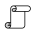
\includegraphics[width=13.9bp]{icone-page.png}};
    \node[anchor=base east,inner sep=0pt,font=\fontsize{6}{7}\selectfont] at ($(O)+(567,20.95)$) {\thepage\,/\,\pageref*{LastPage}};
  \end{tikzpicture}}

% ------------------------------------------------------------------ titres
% Saut de page seulement si la place restante est insuffisante (n'introduit
% pas de point de coupure « préférentiel », contrairement à needspace)
\makeatletter
\newcommand{\BesoinPlace}[1]{\par\begingroup\setlength{\dimen@}{#1}%
  \dimen@ii\pagegoal\advance\dimen@ii-\pagetotal
  \ifdim\dimen@>\dimen@ii\ifdim\dimen@ii>\z@\vfil\fi\break\fi\endgroup}
\makeatother
\newcommand{\TitrePrincipal}[2]{%
  \vspace*{-7.1bp}%
  {\centering\caladea\fontsize{21.6}{24}\selectfont\color{titreBleu}#1\par}%
  \vspace{-4.9bp}%
  {\centering\color{filetBleu}\rule{471.7bp}{0.6bp}\par}%
  \vspace{9.4bp}%
  {\centering\fontsize{14}{16}\selectfont\bfseries #2\par}%
  \vspace{2.0bp}}

% Bandeau de section : barre 5,4 bp + aplat jusqu'à 508,4 bp, hauteur 20,6 bp
\newcommand{\Section}[2]{%
  \par\BesoinPlace{9\baselineskip}\vspace{\EspAvantSection}%
  \noindent\begin{tikzpicture}[x=1bp,y=1bp,baseline=(b)]
    \coordinate (b) at (0,0);
    \fill[bandeBleu] (0,0) rectangle (508.4,20.6);
    \fill[secBleu] (0,0) rectangle (5.4,20.6);
    \node[anchor=base west,inner sep=0pt,text=secBleu,
          font=\carlito\fontsize{20}{22}\selectfont] at (12.1,2.7) {#1. #2};
  \end{tikzpicture}\par\vskip\EspApresSection\relax}

\newcommand{\SousSection}[2]{%
  \par\ifdim\lastskip=\EspApresSection\vskip-\CorrSousSection\relax\fi
  \BesoinPlace{7\baselineskip}\vspace{\EspAvantSousSection}%
  \noindent\hspace*{65.2bp}{\carlito\fontsize{15}{17}\selectfont\color{secBleu}#1. %
  \tikz[baseline=(t.base)]{\node[inner sep=0pt](t){#2};
    \draw[secBleu,line width=0.6bp] ($(t.base west)+(0,-2.3bp)$) -- ($(t.base east)+(0,-2.3bp)$);}}%
  \par\vspace{\EspApresSousSection}}
\newcommand{\EspAvantSection}{44.5bp}
\newlength{\EspApresSection}\setlength{\EspApresSection}{3.9001bp}% marqueur : sert à détecter une sous-section qui suit immédiatement
\newlength{\CorrSousSection}\setlength{\CorrSousSection}{16.1bp}
\newcommand{\EspAvantSousSection}{19bp}
\newcommand{\EspApresSousSection}{6.3bp}

% ------------------------------------------------------------------ boîtes de résultats
\newcommand{\Resultat}[2][]{%
  \begin{center}
    \setlength{\fboxrule}{1pt}\setlength{\fboxsep}{5pt}%
    \fcolorbox{bleuConnu}{white}{$\displaystyle\thickmuskip=12mu\medmuskip=7mu #2$}%
    \if\relax\detokenize{#1}\relax\else\\[1pt]#1\fi
  \end{center}}

% ------------------------------------------------------------------ tableaux
\newcolumntype{C}[1]{>{\centering\arraybackslash}m{#1}}
\newcolumntype{L}[1]{>{\raggedright\arraybackslash}m{#1}}
\newcommand{\entete}{\rowcolor{bandeBleu}}
\newcommand{\haut}{\rule[-9pt]{0pt}{24pt}}

% ------------------------------------------------------------------ styles TikZ
\tikzset{
  barre/.style={line width=2.2pt,color=noirBarre},
  cote/.style={draw=grisCote,line width=0.4pt},
  fcote/.style={cote,{To[length=2.6pt,width=3.2pt]}-{To[length=2.6pt,width=3.2pt]}},
  axe/.style={draw=black!45,line width=0.4pt,dash pattern=on 4pt off 1.5pt on 0.6pt off 1.5pt,-{To[length=4pt,width=5pt]}},
  inconnue/.style={rougeInc,line width=1.6pt,-{Stealth[length=7pt,width=6.4pt]}},
  connue/.style={bleuConnu,line width=1.6pt,-{Stealth[length=7pt,width=6.4pt]}},
  charge/.style={black,line width=1.4pt,-{Stealth[length=6.5pt,width=5.8pt]}},
  torseur/.style={black,line width=1.4pt,-{Stealth[length=6.5pt,width=5.8pt]}},
  repere/.style={black,line width=0.45pt},
  coupure/.style={rougeInc,line width=0.6pt},
  diag/.style={fill=aplat,fill opacity=0.92,draw=black,line width=0.35pt},
  pt/.style={font=\fontsize{6.5}{7}\selectfont,inner sep=1.5pt},
  gros/.style={font=\fontsize{12}{14}\selectfont,inner sep=2pt},
  moyen/.style={font=\fontsize{9}{10}\selectfont,inner sep=1.5pt},
  petit/.style={font=\fontsize{7.5}{8}\selectfont,inner sep=1.5pt},
  diaglbl/.style={font=\fontsize{8.5}{9.5}\selectfont,inner sep=1.5pt},
}
% Symbole de repère local en L : coin = origine, bras long = x (angle #2), bras court = y
\newcommand{\repereL}[3][0.75]{%
  \draw[repere] ($#2+(#3+90:0.27)$) -- #2 -- ($#2+(#3:#1)$);}
% Articulation : petit cercle (avec sol hachuré si #2 = sol)
\newcommand{\articulation}[2][]{%
  \if\relax\detokenize{#1}\relax\else
    \fill[pattern={Lines[angle=45,distance=2.6pt,line width=0.35pt]}] ($#2+(-0.68,-0.39)$) rectangle ($#2+(0.68,-0.09)$);
    \draw[line width=0.5pt] ($#2+(-0.68,-0.09)$) -- ($#2+(0.68,-0.09)$);
  \fi
  \draw[fill=white,line width=0.6pt] #2 circle (0.085);}
% Appui simple : triangle, rouleaux, sol hachuré
\newcommand{\appuiSimple}[1]{%
  \shade[top color=black!75,bottom color=black!8,draw=black,line width=0.4pt]
     #1 -- ++(-0.28,-0.34) -- ++(0.56,0) -- cycle;
  \draw[fill=white,line width=0.45pt] ($#1+(-0.14,-0.405)$) circle (0.065);
  \draw[fill=white,line width=0.45pt] ($#1+(0.14,-0.405)$) circle (0.065);
  \draw[line width=0.5pt] ($#1+(-0.36,-0.47)$) -- ($#1+(0.36,-0.47)$);
  \fill[pattern={Lines[angle=45,distance=2.6pt,line width=0.35pt]}] ($#1+(-0.36,-0.7)$) rectangle ($#1+(0.36,-0.47)$);}
% Coupure Σ sur une barre horizontale (point #1, étiquette #2), tournée de #3 degrés
\newcommand{\coupure}[3][0]{%
  \begin{scope}[shift={#2},rotate=#1]
    \draw[coupure] (-0.06,0.5) .. controls (-0.14,0.18) and (0.26,0.02) .. (0.27,-0.42);
    \node[rougeInc,moyen,font=\fontsize{10}{11}\selectfont] at (0.08,-0.62) {#3};
  \end{scope}}
% Face de coupure hachurée (centre #1, rotation #2)
\newcommand{\faceCoupure}[2][0]{%
  \begin{scope}[shift={#2},rotate=#1]
    \fill[white] (-0.06,-0.27) rectangle (0.08,0.27);
    \fill[pattern={Lines[angle=45,distance=1.7pt,line width=0.3pt]}] (-0.06,-0.27) rectangle (0.08,0.27);
    \draw[line width=0.35pt] (-0.06,-0.27) rectangle (0.08,0.27);
  \end{scope}}
% Signe cerclé ⊕ / ⊖ dans une zone de diagramme
\newcommand{\signe}[2]{%
  \node[circle,draw=black,line width=0.45pt,fill=white,inner sep=0pt,minimum size=8.4pt,
        font=\fontsize{8.5}{8.5}\selectfont\bfseries] at #1 {$#2$};}


\begin{document}

\TitrePrincipal{Torseur de cohésion des portiques plans isostatiques}{Portique à force oblique (S\textsubscript{4}) — CORRECTION}

\Sq{} ne porte qu'\textbf{une seule charge}, la force $F$ appliquée en C, mais elle est \textbf{oblique}. C'est le fait marquant de cette structure, et il commande toute la correction : tant que la force n'est pas projetée, aucune équation d'équilibre ne peut s'écrire proprement. La méthode est donc celle de la \textbf{projection puis de la superposition}. La convention de signe du cours ne change pas : $\dMdx = -T(x)$.

Une convention de lecture, valable dans tout ce corrigé : la force oblique $F$ n'est dessinée telle quelle que sur l'énoncé. Partout ailleurs, elle est remplacée par ses deux composantes $F_x$ et $F_y$ — ce sont elles, et non $F$, qui portent les bras de levier. Les diagrammes, eux, sont reportés selon le $y$ local de chaque barre : c'est le symbole $\oplus$ ou $\ominus$ qui porte le signe, et la fibre tendue est du côté opposé au diagramme.

% =====================================================================
\Section{1}{Mise en place}
\SousSection{1.1}{Énoncé}

Le portique \Sq{} est formé de deux barres. Le \textbf{poteau} AB, vertical, de hauteur $H$, est \textbf{articulé au sol} en A. La \textbf{poutre} CD, horizontale, le traverse au nœud B : elle déborde de $L$ à gauche — la partie CB est \textbf{en console}, son extrémité C est libre — et de $2L$ à droite, jusqu'à l'\textbf{appui simple} D. L'ensemble porte une force unique $F$, appliquée en C, dirigée vers le haut et vers la droite, et inclinée de $\alpha$ \textbf{par rapport à la verticale}.

\begin{center}
\begin{tikzpicture}[x=1cm,y=1cm]
  \def\L{2.6}\def\H{4.16}
  \coordinate (A) at (0,0); \coordinate (B) at (0,\H);
  \coordinate (C) at (-\L,\H); \coordinate (D) at (2*\L,\H);
  % repère global
  \draw[axe] (0,0) -- (0,\H+1.45) node[above left=-1pt,font=\fontsize{11}{12}\selectfont] {$Y$};
  \draw[axe] (0,0) -- (2*\L+2.1,0) node[below=1pt,font=\fontsize{11}{12}\selectfont] {$X$};
  % cotes
  \foreach \xx in {-\L,0,2*\L} \draw[cote] (\xx,\H+0.2) -- (\xx,\H+1.1);
  \draw[fcote] (-\L,\H+0.95) -- node[above,petit] {$L$} (0,\H+0.95);
  \draw[fcote] (0,\H+0.95) -- node[above,petit] {$2L$} (2*\L,\H+0.95);
  \draw[cote] (2*\L+0.55,\H) -- (2*\L+1.7,\H);
  \draw[fcote] (2*\L+1.4,0) -- node[above,sloped,petit] {$H$} (2*\L+1.4,\H);
  % barres et liaisons
  \draw[barre] (C) -- (D);
  \draw[barre] (A) -- (B);
  \articulation[sol]{(A)}
  \appuiSimple{(D)}
  % repères locaux
  \repereL{(-0.95*\L,\H+0.16)}{0}
  \repereL{(0.3*\L,\H+0.16)}{0}
  \repereL{(-0.17,0.55*\H)}{90}
  % force oblique
  \draw[black!55,line width=0.4pt,densely dashed] (C) -- ++(0,-1.5);
  \draw[charge] ($(C)+(225:1.8)$) -- (C);
  \node[gros,text=bleuConnu,anchor=north east] at ($(C)+(225:1.8)$) {$F$};
  \draw[line width=0.4pt] ($(C)+(270:0.9)$) arc[start angle=270,end angle=225,radius=0.9];
  \node[font=\fontsize{9.5}{10}\selectfont] at ($(C)+(247.5:1.14)$) {$\alpha$};
  % étiquettes
  \node[pt,anchor=south east] at ($(C)+(-0.05,0.05)$) {$C$};
  \node[pt,anchor=north west] at (0.1,\H-0.08) {$B$};
  \node[pt,anchor=south west] at ($(D)+(0.1,0.07)$) {$D$};
  \node[pt,anchor=south west] at (0.12,0.07) {$A$};
  \node[font=\fontsize{12}{14}\selectfont] at (1.0*\L,0.45*\H) {$(S_4)$};
\end{tikzpicture}
\end{center}

Le chargement se résume à l'intensité $F$ et à l'angle $\alpha$. Comme $\alpha$ est mesuré \textbf{depuis la verticale}, c'est le cosinus qui donne la composante verticale et le sinus la composante horizontale :
\[ F_x \;=\; F\sin\alpha \qquad\qquad F_y \;=\; F\cos\alpha \]
Pour tout $\alpha$ compris entre 0 et 90°, les deux composantes sont \textbf{positives} : la force pousse vers la droite et tire vers le haut. Ce sont elles qui serviront dans toutes les équations d'équilibre.

\textbf{Deux niveaux de repère}, comme sur toute structure à plusieurs barres. Un repère global $(X,Y)$ unique, d'origine A, l'axe $Y$ confondu avec le poteau : il sert au principe fondamental de la statique et aux réactions. Et un repère local $(x,y)$ \textbf{par barre}, celui que porte le petit symbole en L — le coin marque l'origine, le bras long porte $x$, le bras court porte $y$. C'est lui, et lui seul, qui oriente le torseur de cohésion de sa barre.

Ceux du sujet : sur \textbf{CB} et sur \textbf{BD}, $x$ va de gauche à droite et $y$ vers le haut ; sur \textbf{AB}, $x$ monte de A vers B et $y$ pointe vers la gauche. Dans les trois cas, $y$ s'obtient en tournant $x$ de $+90°$ — c'est ce qui garantira que les diagrammes se raccordent d'eux-mêmes autour du nœud B. La poutre porte deux symboles, un de chaque côté du nœud : la console CB et la travée BD sont donc traitées comme deux barres, chacune avec sa propre origine, C pour l'une, B pour l'autre.

\SousSection{1.2}{Les liaisons et le degré d'hyperstaticité}

Deux liaisons extérieures. En A, une \textbf{articulation} — le petit cercle posé sur les hachures : elle bloque les deux translations mais laisse la rotation libre, donc deux inconnues, $A_x$ et $A_y$, et \textbf{aucun moment}. En D, un \textbf{appui simple} — le triangle sur rouleaux : il ne bloque que la translation verticale, donc une seule inconnue, $D_y$.

Le nœud B est une liaison \textbf{intérieure} : un encastrement, trois extrémités de barre simplement jointives — la console, la travée et le poteau. \textbf{Aucun symbole n'y est dessiné — l'absence de cercle est la notation.} Il n'apporte donc aucune équation supplémentaire. Mais trois branches s'y rejoignent, et non deux : $N$, $T$ et $M$ ne passent pas d'une barre à l'autre, ils \textbf{s'y répartissent}. L'extrémité C, elle, est libre — chargée, mais libre : ce n'est pas une liaison du tout.
\[ h \;=\; 3 - (2 + 1) \;=\; 0 \]
La structure est isostatique : les trois équations d'équilibre suffisent.

% =====================================================================
\Section{2}{Réactions d'appui}
\SousSection{2.1}{Une force oblique : on projette, puis on superpose}

$F$ est unique, donc rien n'obligerait a priori à superposer. Mais une fois projetée, plus rien ne lie $F_x$ à $F_y$ : leur rapport ne dépend que de $\alpha$, qui n'est pas donné. Les réactions et le torseur de cohésion étant des fonctions \textbf{linéaires} du chargement, on peut découper :

\begin{center}
\newcommand{\mini}[1]{%
  \draw[line width=1.5pt,noirBarre] (-0.95,1.52) -- (1.9,1.52);
  \draw[line width=1.5pt,noirBarre] (0,0) -- (0,1.52);
  \fill[pattern={Lines[angle=45,distance=2.2pt,line width=0.3pt]}] (-0.36,-0.26) rectangle (0.36,-0.06);
  \draw[line width=0.4pt] (-0.36,-0.06) -- (0.36,-0.06);
  \draw[fill=white,line width=0.5pt] (0,0) circle (0.06);
  \shade[top color=black!75,bottom color=black!8,draw=black,line width=0.3pt] (1.9,1.52) -- ++(-0.15,-0.2) -- ++(0.3,0) -- cycle;
  \draw[line width=0.4pt] (1.7,1.27) -- (2.1,1.27);
  \fill[pattern={Lines[angle=45,distance=2.2pt,line width=0.3pt]}] (1.7,1.13) rectangle (2.1,1.27);
  #1}
\begin{tikzpicture}[x=1cm,y=1cm]
  \begin{scope}
    \mini{\draw[charge,line width=1.2pt] ($(-0.95,1.52)+(225:0.95)$) -- (-0.95,1.52);
          \node[moyen,text=bleuConnu,anchor=north east] at ($(-0.95,1.52)+(225:0.95)$) {$F$};}
    \node[font=\fontsize{10}{11}\selectfont] at (0.5,-0.6) {$(S_4)$};
  \end{scope}
  \node[font=\fontsize{16}{16}\selectfont] at (2.85,0.8) {$=$};
  \begin{scope}[xshift=5.0cm]
    \mini{\draw[charge,line width=1.2pt] (-1.95,1.52) -- (-0.95,1.52);
          \node[moyen,text=bleuConnu,anchor=south] at (-1.5,1.55) {$F_x$};}
    \node[font=\fontsize{10}{11}\selectfont] at (0.5,-0.6) {$(S_x)$};
  \end{scope}
  \node[font=\fontsize{16}{16}\selectfont] at (7.85,0.8) {$+$};
  \begin{scope}[xshift=10.0cm]
    \mini{\draw[charge,line width=1.2pt] (-0.95,0.52) -- (-0.95,1.52);
          \node[moyen,text=bleuConnu,anchor=east] at (-0.97,0.85) {$F_y$};}
    \node[font=\fontsize{10}{11}\selectfont] at (0.5,-0.6) {$(S_y)$};
  \end{scope}
\end{tikzpicture}
\end{center}

On étudie $(S_x)$, chargée par $F_x$ seule, puis $(S_y)$, chargée par $F_y$ seule. Chacune est simple : une force parallèle à un axe, un seul bras de levier à écrire. Les réactions de \Sq{} s'obtiennent ensuite par simple addition.

Ce détour n'est pas un luxe. Sur cette structure, $F_x$ et $F_y$ \textbf{ne chargent pas les mêmes barres} : la composante horizontale fléchit le poteau et laisse la console indifférente, la composante verticale fait exactement l'inverse. Les écrire séparément, c'est voir les deux mécanismes avant de les additionner.

\SousSection{2.2}{On isole $(S_x)$}

Les appuis disparaissent, remplacés par leurs trois inconnues, en rouge et toutes dessinées dans le sens positif du repère global — c'est une convention d'écriture, pas une prévision. Les bras de levier utiles au calcul des moments en A sont cotés.

\begin{center}
\begin{tikzpicture}[x=1cm,y=1cm]
  \def\L{2.2}\def\H{3.52}
  \coordinate (A) at (0,0); \coordinate (B) at (0,\H);
  \coordinate (C) at (-\L,\H); \coordinate (D) at (2*\L,\H);
  % cotes
  \draw[cote] (0,\H+0.2) -- (0,\H+1.0); \draw[cote] (2*\L,\H+0.2) -- (2*\L,\H+1.0);
  \draw[fcote] (0,\H+0.85) -- node[above,petit] {$2L$} (2*\L,\H+0.85);
  \draw[cote] (0.15,0) -- (0.62*\L,0);
  \draw[fcote] (0.5*\L,0) -- node[above,sloped,petit] {$H$} (0.5*\L,\H-0.06);
  % structure
  \draw[barre] (C) -- (D);
  \draw[barre] (A) -- (B);
  \draw[fill=white,line width=0.6pt] (A) circle (0.085);
  % charge
  \draw[charge] (-\L-1.2,\H) -- (C);
  \node[gros,text=bleuConnu,anchor=south] at (-\L-0.65,\H+0.05) {$F_x$};
  % inconnues
  \draw[inconnue] (-1.3,0) -- (-0.1,0);
  \node[gros,text=rougeInc,anchor=south] at (-1.0,0.05) {$A_x$};
  \draw[inconnue] (0,-1.3) -- (0,-0.1);
  \node[gros,text=rougeInc,anchor=east] at (-0.05,-1.0) {$A_y$};
  \draw[inconnue] (2*\L,\H-1.3) -- (2*\L,\H-0.05);
  \node[gros,text=rougeInc,anchor=west] at (2*\L+0.05,\H-1.0) {$D_y$};
  % étiquettes
  \node[pt,anchor=south east] at ($(C)+(-0.03,0.25)$) {$C$};
  \node[pt,anchor=north west] at (0.1,\H-0.08) {$B$};
  \node[pt,anchor=south west] at ($(D)+(0.08,0.07)$) {$D$};
  \node[pt,anchor=north west] at (0.1,-0.06) {$A$};
\end{tikzpicture}
\end{center}

PFS :
\[ \left\{\begin{array}{r@{\;\;}c@{\;\;}r@{\;\;=\;\;}l}
  \Sigma F_x = 0 & \Longrightarrow & A_x + F_x & 0\\[3pt]
  \Sigma F_y = 0 & \Longrightarrow & A_y + D_y & 0\\[3pt]
  \Sigma M_{/A} = 0 & \Longrightarrow & D_y\cdot 2L - F_x\cdot H & 0
\end{array}\right. \]
\Resultat{\left\{\begin{array}{l@{\;\;=\;\;}l}
  A_x & -F_x\\[3pt]
  A_y & -\dfrac{H F_x}{2L}\\[9pt]
  D_y & \dfrac{H F_x}{2L}
\end{array}\right.}

Deux choses à lire dans ces équations. D'abord le bras de levier de $F_x$ par rapport à A : c'est la \textbf{hauteur} $H$, pas la portée $L$. Le bras de levier est une distance mesurée perpendiculairement à la force ; $F_x$ étant horizontale, seule la position verticale de son point d'application compte, et le porte-à-faux $L$ n'y entre pas.

Ensuite, $A_y$ et $D_y$ sont égales et opposées : elles forment un \textbf{couple}, de bras $2L$, et c'est ce couple qui équilibre le moment $H\,F_x$. L'articulation ne pouvant reprendre aucun moment, il fallait bien que les deux appuis se partagent le travail. Toute la composante horizontale, elle, descend dans l'articulation : $A_x = -F_x$.

\SousSection{2.3}{On isole $(S_y)$}

Même démarche, avec $F_y$ pour unique chargement. Cette fois c'est la portée $L$ de la console qui donne le bras de levier, et la hauteur $H$ qui n'entre pas : $F_y$ est verticale, seule la position horizontale de son point d'application compte.

\begin{center}
\begin{tikzpicture}[x=1cm,y=1cm]
  \def\L{2.2}\def\H{3.52}
  \coordinate (A) at (0,0); \coordinate (B) at (0,\H);
  \coordinate (C) at (-\L,\H); \coordinate (D) at (2*\L,\H);
  % cotes
  \foreach \xx in {-\L,0,2*\L} \draw[cote] (\xx,\H+0.2) -- (\xx,\H+1.0);
  \draw[fcote] (-\L,\H+0.85) -- node[above,petit] {$L$} (0,\H+0.85);
  \draw[fcote] (0,\H+0.85) -- node[above,petit] {$2L$} (2*\L,\H+0.85);
  % structure
  \draw[barre] (C) -- (D);
  \draw[barre] (A) -- (B);
  \draw[fill=white,line width=0.6pt] (A) circle (0.085);
  % charge
  \draw[charge] (-\L,\H-1.2) -- (C);
  \node[gros,text=bleuConnu,anchor=east] at (-\L-0.05,\H-0.75) {$F_y$};
  % inconnues
  \draw[inconnue] (-1.3,0) -- (-0.1,0);
  \node[gros,text=rougeInc,anchor=south] at (-1.0,0.05) {$A_x$};
  \draw[inconnue] (0,-1.3) -- (0,-0.1);
  \node[gros,text=rougeInc,anchor=east] at (-0.05,-1.0) {$A_y$};
  \draw[inconnue] (2*\L,\H-1.3) -- (2*\L,\H-0.05);
  \node[gros,text=rougeInc,anchor=west] at (2*\L+0.05,\H-1.0) {$D_y$};
  % étiquettes
  \node[pt,anchor=south east] at ($(C)+(-0.06,0.05)$) {$C$};
  \node[pt,anchor=north west] at (0.1,\H-0.08) {$B$};
  \node[pt,anchor=south west] at ($(D)+(0.08,0.07)$) {$D$};
  \node[pt,anchor=north west] at (0.1,-0.06) {$A$};
\end{tikzpicture}
\end{center}

PFS :
\[ \left\{\begin{array}{r@{\;\;}c@{\;\;}r@{\;\;=\;\;}l}
  \Sigma F_x = 0 & \Longrightarrow & A_x & 0\\[3pt]
  \Sigma F_y = 0 & \Longrightarrow & A_y + D_y + F_y & 0\\[3pt]
  \Sigma M_{/A} = 0 & \Longrightarrow & D_y\cdot 2L - F_y\cdot L & 0
\end{array}\right. \]
\Resultat{\left\{\begin{array}{l@{\;\;=\;\;}l}
  A_x & 0\\[3pt]
  A_y & -\dfrac{3F_y}{2}\\[9pt]
  D_y & \dfrac{F_y}{2}
\end{array}\right.}

$A_y$ est négative : le sol \textbf{retient le poteau vers le bas}. Une articulation le peut, elle travaille dans les deux sens. Physiquement, la force de levage appliquée en C fait basculer la poutre autour de B ; l'extrémité D tend à descendre, l'appui simple la repousse vers le haut, et le poteau doit encaisser la somme des deux — d'où $3F_y/2$. Noter enfin que $A_x = 0$ est un \textbf{résultat} : c'est la première équation du PFS qui le démontre.

\BesoinPlace{185bp}
\SousSection{2.4}{Superposition}

Les réactions s'ajoutent, colonne par colonne :

\begin{center}
\arrayrulecolor{grisCote}
\begin{tabular}{|C{2.6cm}|C{2.6cm}|C{4.4cm}|C{4.4cm}|}
  \hline
  \entete & $A_x$ & $A_y$ & $D_y$ \\ \hline
  \haut $(S_x)$ & $-F_x$ & $-\dfrac{HF_x}{2L}$ & $\dfrac{HF_x}{2L}$ \\ \hline
  \haut $(S_y)$ & $0$ & $-\dfrac{3F_y}{2}$ & $\dfrac{F_y}{2}$ \\ \hline
  \haut \textbf{\Sq} & $-F_x$ & $-\dfrac{3F_y}{2}-\dfrac{HF_x}{2L}$ & $\dfrac{F_y}{2}+\dfrac{HF_x}{2L}$ \\ \hline
\end{tabular}
\arrayrulecolor{black}
\end{center}

\Resultat[avec $F_x = F\sin\alpha$ et $F_y = F\cos\alpha$]{\left\{\begin{array}{l@{\;\;=\;\;}l}
  A_x & -F_x\\[3pt]
  A_y & -\left(\dfrac{3F_y}{2}+\dfrac{HF_x}{2L}\right)\\[9pt]
  D_y & \dfrac{F_y}{2}+\dfrac{HF_x}{2L}
\end{array}\right.}

Tout s'exprime en fonction de $F$, de $\alpha$ et du seul rapport $H/L$. $D_y$ est positive pour tout $\alpha$ : l'appui simple pousse toujours vers le haut. $A_y$ est toujours négative : le pied du poteau est toujours retenu vers le bas.

\SousSection{2.5}{Vérification de l'équilibre}

On réinjecte les valeurs trouvées dans \Sq{} complète, en prenant les moments en un point \textbf{différent} de celui qui a servi à les calculer — sinon le contrôle serait circulaire. Par rapport à D, le bras de levier de $A_x$ vaut $H$, celui de $A_y$ vaut $2L$, celui de $F_y$ vaut $3L$ ; quant à $F_x$, elle est portée par l'horizontale CD, qui passe par D : son bras de levier est nul.
\[ \Sigma M_{/D} \;=\; H\cdot A_x \;-\; 2L\cdot A_y \;-\; 3L\cdot F_y \;=\; -HF_x \;+\; \left(3LF_y + HF_x\right) \;-\; 3LF_y \;=\; 0 \ok \]
Les deux équations de forces se vérifient de même : $A_x + F_x = 0$ et $A_y + D_y + F_y = -\frac{3F_y}{2} + \frac{F_y}{2} + F_y = 0$, les termes en $HF_x/(2L)$ s'éliminant. \Sq{} est bien en équilibre.

% =====================================================================
\Section{3}{Le torseur de cohésion}
\SousSection{3.1}{Le système en équilibre, et les coupures}

On redessine la structure en équilibre. Les appuis ont disparu — il n'en reste aucun symbole —, les réactions sont bleues puisqu'elles sont désormais connues, et chacune est tracée dans le sens où elle s'applique réellement, avec une grandeur positive : $A_x$ et $A_y$ étant négatives, elles sont dessinées vers la gauche et vers le bas.

On travaille désormais directement sur \Sq{}, avec les réactions sommées : par linéarité, le torseur de \Sq{} est la somme de ceux de $(S_x)$ et de $(S_y)$, et l'on verra sur chaque tronçon laquelle des deux composantes agit.

C'est sur ce système en équilibre — et sur lui seul — que se placent les coupures. Il en faut \textbf{au moins une par barre} : une abscisse ne se poursuit pas d'une barre à l'autre, puisqu'elles n'ont pas le même repère local. Ici, trois : $\Sigma_1$ sur la console, $\Sigma_2$ sur la travée, $\Sigma_3$ sur le poteau. Les repères locaux figurent obligatoirement sur cette figure : sans eux, « à droite de $\Sigma_2$ » ne désignerait rien.

\begin{center}
\begin{tikzpicture}[x=1cm,y=1cm]
  \def\L{2.6}\def\H{4.16}
  \coordinate (A) at (0,0); \coordinate (B) at (0,\H);
  \coordinate (C) at (-\L,\H); \coordinate (D) at (2*\L,\H);
  % repère global
  \draw[axe] (0,0) -- (0,\H+1.2) node[above left=-1pt,font=\fontsize{11}{12}\selectfont] {$Y$};
  \draw[axe] (0,0) -- (2*\L+2.1,0) node[below=1pt,font=\fontsize{11}{12}\selectfont] {$X$};
  % barres
  \draw[barre] (C) -- (D);
  \draw[barre] (A) -- (B);
  % repères locaux
  \repereL{(-0.95*\L,\H+0.16)}{0}
  \repereL{(0.3*\L,\H+0.16)}{0}
  \repereL{(-0.17,0.55*\H)}{90}
  % charges
  \draw[charge] (-\L-1.2,\H) -- (C);
  \node[gros,text=bleuConnu,anchor=south] at (-\L-0.7,\H+0.05) {$F_x$};
  \draw[charge] (-\L,\H-1.2) -- (C);
  \node[gros,text=bleuConnu,anchor=east] at (-\L-0.05,\H-0.8) {$F_y$};
  % réactions connues
  \draw[connue] (1.35,0) -- (0.06,0);
  \node[gros,text=bleuConnu,anchor=south] at (0.8,0.05) {$F_x$};
  \draw[connue] (0,-0.06) -- (0,-1.35);
  \node[text=bleuConnu,anchor=west,font=\fontsize{10.5}{12}\selectfont] at (0.1,-0.95) {$\dfrac{3F_y}{2}+\dfrac{HF_x}{2L}$};
  \draw[connue] (2*\L,\H-1.4) -- (2*\L,\H-0.05);
  \node[text=bleuConnu,anchor=west,font=\fontsize{10.5}{12}\selectfont] at (2*\L+0.08,\H-1.0) {$\dfrac{F_y}{2}+\dfrac{HF_x}{2L}$};
  % coupures
  \coupure{(-0.42*\L,\H)}{$\Sigma_1$}
  \coupure{(1.35*\L,\H)}{$\Sigma_2$}
  \coupure[90]{(0,0.3*\H)}{$\Sigma_3$}
  % étiquettes
  \node[pt,anchor=south east] at ($(C)+(-0.05,0.05)$) {$C$};
  \node[pt,anchor=north west] at (0.1,\H-0.08) {$B$};
  \node[pt,anchor=south west] at ($(D)+(0.08,0.07)$) {$D$};
  \node[pt,anchor=north east] at (-0.08,-0.06) {$A$};
\end{tikzpicture}
\end{center}

Sur chaque barre, $x$ part de l'origine de son repère local : de C sur CB ($0 \le x \le L$), de B sur BD ($0 \le x \le 2L$), de A sur AB ($0 \le x \le H$).

\BesoinPlace{260bp}
\SousSection{3.2}{Tronçon à gauche de $\Sigma_1$ — la console}

Le repère local de la console a son axe $x$ orienté de C vers B : la partie \textbf{à gauche} de la coupure va donc de l'extrémité libre C à la section. C'est le côté le moins chargé, et il ne porte aucune réaction de liaison — seulement les deux composantes de $F$, appliquées en C. Le torseur s'appliquant par définition sur la partie \textbf{à gauche}, il s'applique ici tel quel : étiquettes $N(x)$, $T(x)$, $M(x)$, flèches dans le sens positif du repère.

\noindent\begin{minipage}[c]{0.52\textwidth}
\centering
\begin{tikzpicture}[x=1cm,y=1cm]
  \def\s{2.7}
  \draw[barre] (0,0) -- (\s,0);
  \draw[charge] (-1.15,0) -- (-0.02,0);
  \node[gros,text=bleuConnu,anchor=south] at (-0.65,0.05) {$F_x$};
  \draw[charge] (0,-1.15) -- (0,-0.02);
  \node[gros,text=bleuConnu,anchor=east] at (-0.05,-0.75) {$F_y$};
  \faceCoupure{(\s,0)}
  \draw[torseur] (\s+0.08,0) -- (\s+1.15,0) node[right,gros] {$N(x)$};
  \draw[torseur] (\s,0.3) -- (\s,1.25) node[above,gros] {$T(x)$};
  \draw[torseur] ($(\s,0)+(-62:0.5)$) arc[start angle=-62,end angle=62,radius=0.5];
  \node[gros,anchor=north west] at (\s+0.3,-0.45) {$M(x)$};
  \node[pt,anchor=north west] at (\s+0.1,-0.2) {$M$};
  \node[pt,anchor=south east] at (-0.05,0.06) {$C$};
  % cote
  \draw[cote] (0,-1.25) -- (0,-1.6); \draw[cote] (\s,-0.35) -- (\s,-1.6);
  \draw[fcote] (0,-1.45) -- node[above,petit] {$x$} (\s,-1.45);
\end{tikzpicture}
\end{minipage}\hfill
\begin{minipage}[c]{0.46\textwidth}
\[ \left\{\begin{array}{r@{\;\;=\;\;}l}
  N(x) + F_x & 0\\[3pt]
  T(x) + F_y & 0\\[3pt]
  M(x) - F_y\cdot x & 0
\end{array}\right. \]
\Resultat[avec $0 \;\le\; x \;\le\; L$]{\left\{\begin{array}{l@{\;\;=\;\;}l}
  N_{CB}(x) & -F_x\\[3pt]
  T_{CB}(x) & -F_y\\[3pt]
  M_{CB}(x) & F_y\, x
\end{array}\right.}
\end{minipage}

Contrôle : $\dMdx = F_y = -T(x) \ok$. Les deux composantes jouent des rôles bien séparés. $F_x$ est portée par l'axe même de la console : son bras de levier par rapport à n'importe quelle section est nul, elle ne crée qu'une \textbf{compression} constante. $F_y$ seule fléchit la console : tranchant constant, moment \textbf{linéaire}, nul en C — extrémité libre — et égal à $LF_y$ en B. Il est positif : la force soulève le bout de la console, et c'est la fibre inférieure qui est tendue. Noter qu'en C le tranchant et l'effort normal ne s'annulent pas : l'extrémité est libre mais chargée, et le torseur y reproduit, au signe près, la force appliquée.

\BesoinPlace{270bp}
\SousSection{3.3}{Tronçon à droite de $\Sigma_2$ — la travée}

Sur la travée, la partie à gauche de la coupure emporterait la console, la force $F$, le poteau et les réactions en A. On prend donc la partie \textbf{à droite} : de la section jusqu'à l'appui D. Elle ne porte que la réaction $D_y$. Le torseur s'appliquant par définition sur la partie \textbf{à gauche}, c'est son \textbf{opposé} qui s'applique ici : étiquettes $-N(x)$, $-T(x)$, $-M(x)$, flèches inchangées dans le sens positif du repère.

\noindent\begin{minipage}[c]{0.48\textwidth}
\[ \left\{\begin{array}{r@{\;\;=\;\;}l}
  -N(x) & 0\\[3pt]
  -T(x) + \left(\dfrac{F_y}{2}+\dfrac{HF_x}{2L}\right) & 0\\[9pt]
  -M(x) + \left(\dfrac{F_y}{2}+\dfrac{HF_x}{2L}\right)(2L-x) & 0
\end{array}\right. \]
\Resultat[avec $0 \;\le\; x \;\le\; 2L$]{\left\{\begin{array}{l@{\;\;=\;\;}l}
  N_{BD}(x) & 0\\[3pt]
  T_{BD}(x) & \dfrac{F_y}{2}+\dfrac{HF_x}{2L}\\[9pt]
  M_{BD}(x) & \dfrac{(LF_y + HF_x)(2L-x)}{2L}
\end{array}\right.}
\end{minipage}\hfill
\begin{minipage}[c]{0.50\textwidth}
\centering
\begin{tikzpicture}[x=1cm,y=1cm]
  \def\s{3.0}
  \draw[barre] (0,0) -- (\s,0);
  \faceCoupure{(0,0)}
  \draw[torseur] (-1.25,0) -- (-0.08,0);
  \node[gros,anchor=east] at (-1.25,0) {$-N(x)$};
  \draw[torseur] (0,0.3) -- (0,1.25) node[above,gros] {$-T(x)$};
  \draw[torseur] ($(0,0)+(72:0.5)$) arc[start angle=72,end angle=290,radius=0.5];
  \node[gros,anchor=north east] at (-0.3,-0.45) {$-M(x)$};
  \node[pt,anchor=north west] at (0.1,-0.2) {$M$};
  \draw[connue] (\s,-1.35) -- (\s,-0.05);
  \node[text=bleuConnu,anchor=west,font=\fontsize{10.5}{12}\selectfont] at (\s+0.06,-0.85) {$\dfrac{F_y}{2}+\dfrac{HF_x}{2L}$};
  \node[pt,anchor=south west] at (\s+0.05,0.06) {$D$};
  % cote
  \draw[cote] (0,-0.35) -- (0,-1.75); \draw[cote] (\s,-1.45) -- (\s,-1.75);
  \draw[fcote] (0,-1.6) -- node[above,petit] {$2L-x$} (\s,-1.6);
\end{tikzpicture}
\end{minipage}

Contrôle : $\dMdx = -\dfrac{LF_y + HF_x}{2L} = -T(x) \ok$. Le moment se lit directement sous sa forme factorisée : linéaire, il décroît de $LF_y + HF_x$ en B (pour $x = 0$) à zéro en D, comme il se doit sur un appui simple d'extrémité, où le tranchant vaut $D_y$. Le tranchant ne s'annule nulle part sur la travée : le moment n'y a pas d'extremum intérieur, son maximum est en B. L'effort normal est nul : aucune force horizontale n'agit à droite de B.

\BesoinPlace{300bp}
\SousSection{3.4}{Tronçon à gauche de $\Sigma_3$ — le poteau}

Sur le poteau, l'axe $x$ du repère local monte de A vers B : la partie \textbf{à gauche} de la coupure va du pied A jusqu'à la section. Elle ne porte que les deux réactions de l'articulation, alors que le côté droit emporterait toute la poutre et la force $F$. Le torseur s'y applique donc tel quel : $N(x)$, $T(x)$, $M(x)$.

Tout le travail est dans la projection. Le poteau est vertical, mais son repère local est tourné : $x$ monte, $y$ pointe vers la gauche. La réaction verticale, dirigée vers le bas, est donc portée par $-\vec{x}$ et alimente l'\textbf{effort normal} ; la réaction horizontale, dirigée vers la gauche, est portée par $+\vec{y}$ et alimente le \textbf{tranchant}. Le bras de levier de cette dernière par rapport à la section vaut $x$ : c'est cette fois une distance verticale, mesurée perpendiculairement à une force horizontale. La réaction verticale, elle, passe par toutes les sections du poteau : son bras de levier est nul.

\noindent\begin{minipage}[c]{0.56\textwidth}
\[ \left\{\begin{array}{r@{\;\;=\;\;}l}
  N(x) - \left(\dfrac{3F_y}{2}+\dfrac{HF_x}{2L}\right) & 0\\[9pt]
  T(x) + F_x & 0\\[3pt]
  M(x) - F_x\cdot x & 0
\end{array}\right. \]
\Resultat[avec $0 \;\le\; x \;\le\; H$]{\left\{\begin{array}{l@{\;\;=\;\;}l}
  N_{AB}(x) & \dfrac{3F_y}{2}+\dfrac{HF_x}{2L}\\[9pt]
  T_{AB}(x) & -F_x\\[3pt]
  M_{AB}(x) & F_x\, x
\end{array}\right.}
\end{minipage}\hfill
\begin{minipage}[c]{0.42\textwidth}
\centering
\begin{tikzpicture}[x=1cm,y=1cm]
  \def\s{2.5}
  \draw[barre] (0,0) -- (0,\s);
  \draw[fill=white,line width=0.6pt] (0,0) circle (0.085);
  \draw[connue] (1.2,0) -- (0.11,0);
  \node[gros,text=bleuConnu,anchor=south] at (0.7,0.05) {$F_x$};
  \draw[connue] (0,-0.11) -- (0,-1.25);
  \node[text=bleuConnu,anchor=west,font=\fontsize{10.5}{12}\selectfont] at (0.08,-0.9) {$\dfrac{3F_y}{2}+\dfrac{HF_x}{2L}$};
  \faceCoupure[90]{(0,\s)}
  \draw[torseur] (0,\s+0.08) -- (0,\s+1.15) node[above,gros] {$N(x)$};
  \draw[torseur] (-0.3,\s) -- (-1.25,\s) node[left,gros] {$T(x)$};
  \draw[torseur] ($(0,\s)+(-55:0.5)$) arc[start angle=-55,end angle=55,radius=0.5];
  \node[gros,anchor=west] at (0.5,\s-0.35) {$M(x)$};
  \node[pt,anchor=north east] at (-0.18,\s-0.1) {$M$};
  \node[pt,anchor=north east] at (-0.1,-0.05) {$A$};
  % cote
  \draw[cote] (1.3,0) -- (1.75,0); \draw[cote] (0.62,\s) -- (1.75,\s);
  \draw[fcote] (1.6,0) -- node[above,sloped,petit] {$x$} (1.6,\s);
\end{tikzpicture}
\end{minipage}

Contrôle : $\dMdx = F_x = -T(x) \ok$. $N$ et $T$ sont constants sur tout le poteau : rien n'agit entre A et B. $N$ est positif — le poteau est \textbf{tendu} : la console soulevée tire sur le nœud B, et le pied est retenu au sol. Il est aussi \textbf{fléchi}, mais par la seule composante $F_x$ : le moment croît linéairement, de 0 en A — une articulation ne transmet pas de moment — à sa valeur en tête, pour $x = H$ :
\[ M_{AB}(H) \;=\; H\,F_x \]
$F_y$ n'apparaît que dans l'effort normal : une charge verticale ne fléchit pas le poteau, elle ne fait que le tendre.

\SousSection{3.5}{Récapitulatif et contrôles}

\begin{center}
\arrayrulecolor{grisCote}
\begin{tabular}{|C{3.1cm}|C{1.5cm}|C{2.9cm}|C{2.9cm}|C{4.1cm}|}
  \hline
  \entete \textbf{Barre} & $x$ & $N(x)$ & $T(x)$ & $M(x)$ \\ \hline
  \haut CB\ \ (de C vers B) & $0 \to L$ & $-F_x$ & $-F_y$ & $F_y\,x$ \\ \hline
  \haut BD\ \ (de B vers D) & $0 \to 2L$ & $0$ & $\dfrac{F_y}{2}+\dfrac{HF_x}{2L}$ & $\dfrac{(LF_y+HF_x)(2L-x)}{2L}$ \\ \hline
  \haut AB\ \ (de A vers B) & $0 \to H$ & $\dfrac{3F_y}{2}+\dfrac{HF_x}{2L}$ & $-F_x$ & $F_x\,x$ \\ \hline
\end{tabular}
\arrayrulecolor{black}
\end{center}

\textbf{Sur chaque barre} $\dMdx = -T(x)$. \textbf{Au nœud rigide B}, trois barres se rencontrent et doivent s'équilibrer. En moment, la travée reprend à la fois la console et le poteau :
\[ \Sigma M_{/B} \;=\; -M_{CB}(L) \;+\; M_{BD}(0) \;-\; M_{AB}(H) \;=\; -LF_y \;+\; \left(LF_y + HF_x\right) \;-\; HF_x \;=\; 0 \ok \]
En effort, le poteau étant vertical, ses deux composantes \textbf{échangent leurs rôles} en passant dans la poutre. Son effort normal, vertical, se retrouve dans le saut du tranchant de la poutre ; son tranchant, horizontal, dans le saut de l'effort normal :
\[ T_{BD}(0) - T_{CB}(L) \;=\; \frac{F_y}{2}+\frac{HF_x}{2L} + F_y \;=\; N_{AB} \ok \qquad\qquad N_{BD}(0) - N_{CB}(L) \;=\; 0 + F_x \;=\; -T_{AB} \ok \]

\textbf{Aux extrémités}, $M = 0$ en C, libre, où le torseur se réduit à $N = -F_x$ et $T = -F_y$ ; $M = 0$ en A, articulée, et en D, simplement appuyée, où le tranchant vaut $D_y$.

Deux contrôles de forme, qui se passent de calcul. Le moment de la poutre \textbf{saute en B}, de $LF_y$ à $LF_y + HF_x$ : le saut vaut $HF_x$, exactement le moment que le poteau apporte au nœud — partout ailleurs il est régulier, puisqu'aucune autre force concentrée ni aucun couple n'est appliqué. Et son \textbf{degré} est bien d'un cran au-dessus de celui du tranchant sur chaque barre — linéaire contre constant, partout. Le tranchant ne s'annulant sur aucune barre, le moment n'a pas d'extremum intérieur : son maximum est en bout de barre, en B, côté travée.

Enfin, une remarque qui vaut résultat : $LF_y + HF_x$ n'est autre que le moment de $F$ par rapport à A. C'est la conséquence directe de l'équation des moments en A, qui donne $2L\cdot D_y = LF_y + HF_x$ : le moment de la travée en B, $M_{BD}(0) = 2L\cdot D_y$, est le moment de la force par rapport au pied du poteau.

% =====================================================================
\Section{4}{Les trois diagrammes}

Chaque barre porte son propre diagramme, la valeur étant reportée perpendiculairement à la ligne moyenne, selon le $y$ local de la barre. Les aires sont en aplat bleu, le signe est cerclé dans chaque zone. Les formes sont valables pour tout $\alpha$ compris entre 0 et 90° ; seules les amplitudes relatives en dépendent, et les planches sont tracées pour $H = 1{,}6\,L$ et $\alpha = 45°$, soit $F_x = F_y$.

\vspace{6bp}
\noindent\begin{minipage}[t]{0.333\textwidth}
\centering{\fontsize{11}{12}\selectfont\bfseries Effort normal $N$}\par\vspace{6bp}
\begin{tikzpicture}[x=1cm,y=1cm]
  \def\L{1.5}\def\H{2.4}
  \draw[diag] (-\L,\H) rectangle (0,\H-0.24);
  \draw[diag] (0,0) -- (-0.552,0) -- (-0.552,\H) -- (0,\H) -- cycle;
  \draw[barre,line width=1.9pt] (-\L,\H) -- (2*\L,\H);
  \draw[barre,line width=1.9pt] (0,0) -- (0,\H);
  \repereL[0.45]{(-0.95*\L,\H+0.12)}{0}
  \repereL[0.45]{(1.2*\L,\H+0.12)}{0}
  \repereL[0.45]{(0.32,0.06*\H)}{90}
  \signe{(-0.75*\L,\H-0.12)}{-}
  \signe{(-0.276,0.55*\H)}{+}
  \node[diaglbl,anchor=north] at (-0.75*\L,\H-0.3) {$-F_x$};
  \node[diaglbl,anchor=west] at (0.08,0.45*\H) {$3F_y/2+HF_x/(2L)$};
  \node[pt,anchor=east] at (-\L-0.03,\H) {$C$};
  \node[pt,anchor=south west] at (0.03,\H+0.05) {$B$};
  \node[pt,anchor=west] at (2*\L+0.03,\H) {$D$};
  \node[pt,anchor=north] at (0,-0.05) {$A$};
\end{tikzpicture}
\end{minipage}%
\begin{minipage}[t]{0.333\textwidth}
\centering{\fontsize{11}{12}\selectfont\bfseries Effort tranchant $T$}\par\vspace{6bp}
\begin{tikzpicture}[x=1cm,y=1cm]
  \def\L{1.5}\def\H{2.4}
  \draw[diag] (-\L,\H) rectangle (0,\H-0.28);
  \draw[diag] (0,\H) rectangle (2*\L,\H+0.364);
  \draw[diag] (0,0) rectangle (0.28,\H);
  \draw[barre,line width=1.9pt] (-\L,\H) -- (2*\L,\H);
  \draw[barre,line width=1.9pt] (0,0) -- (0,\H);
  \repereL[0.45]{(-0.95*\L,\H+0.12)}{0}
  \repereL[0.45]{(1.25*\L,\H-0.42)}{0}
  \repereL[0.45]{(-0.14,0.08*\H)}{90}
  \signe{(-0.55*\L,\H-0.14)}{-}
  \signe{(0.75*\L,\H+0.182)}{+}
  \signe{(0.14,0.55*\H)}{-}
  \node[diaglbl,anchor=north] at (-0.55*\L,\H-0.34) {$-F_y$};
  \node[diaglbl,anchor=south] at (\L,\H+0.4) {$F_y/2+HF_x/(2L)$};
  \node[diaglbl,anchor=west] at (0.32,0.3*\H) {$-F_x$};
  \node[pt,anchor=east] at (-\L-0.03,\H) {$C$};
  \node[pt,anchor=north west] at (0.3,\H-0.05) {$B$};
  \node[pt,anchor=west] at (2*\L+0.03,\H) {$D$};
  \node[pt,anchor=north] at (0,-0.05) {$A$};
\end{tikzpicture}
\end{minipage}%
\begin{minipage}[t]{0.333\textwidth}
\centering{\fontsize{11}{12}\selectfont\bfseries Moment fléchissant $M$}\par\vspace{6bp}
\begin{tikzpicture}[x=1cm,y=1cm]
  \def\L{1.5}\def\H{2.4}
  % k = 0,4 cm par F·L  (F_x = F_y, H = 1,6 L)
  \draw[diag] (-\L,\H) -- (0,\H) -- (0,\H+0.4) -- cycle;
  \draw[diag] (0,\H) -- (0,\H+1.04) -- (2*\L,\H) -- cycle;
  \draw[diag] (0,0) -- (0,\H) -- (-0.64,\H) -- cycle;
  \draw[barre,line width=1.9pt] (-\L,\H) -- (2*\L,\H);
  \draw[barre,line width=1.9pt] (0,0) -- (0,\H);
  \repereL[0.45]{(-0.97*\L,\H+0.1)}{0}
  \repereL[0.45]{(1.3*\L,\H+0.12)}{0}
  \repereL[0.45]{(0.14,0.08*\H)}{90}
  \signe{(-0.42*\L,\H+0.13)}{+}
  \signe{(0.45*\L,\H+0.36)}{+}
  \signe{(-0.17,0.75*\H)}{+}
  \node[diaglbl,anchor=south east] at (-0.05,\H+0.4) {$LF_y$};
  \node[diaglbl,anchor=south west] at (0.05,\H+1.04) {$LF_y+HF_x$};
  \node[diaglbl,anchor=east] at (-0.58,\H-0.42) {$HF_x$};
  \node[pt,anchor=east] at (-\L-0.03,\H) {$C$};
  \node[pt,anchor=north west] at (0.06,\H-0.05) {$B$};
  \node[pt,anchor=west] at (2*\L+0.03,\H) {$D$};
  \node[pt,anchor=north] at (0,-0.05) {$A$};
\end{tikzpicture}
\end{minipage}

\SousSection{4.1}{Lecture}

\textbf{Chaque barre a son métier.} La console est comprimée par $F_x$ et fléchie par $F_y$ — c'est la seule barre qui voie les deux composantes. La travée ne porte ni effort normal ni charge : elle transmet à l'appui D, par un tranchant constant, le moment que le nœud lui envoie. Le poteau, enfin, est tendu sur toute sa hauteur, et fléchi par la seule composante horizontale. La planche de $N$ se lit d'un coup d'œil : rien sur la travée, une compression sur la console, une traction dans le poteau.

\textbf{Le signe du moment ne change pas.} Le moment est positif sur les trois barres ; seul le tranchant de la poutre change de signe, en B, de $-F_y$ à $D_y$. Le maximum vaut $LF_y + HF_x$, en B côté travée : c'est la \textbf{valeur de dimensionnement} de la flexion. Avec les projections, il s'écrit $F\,(L\cos\alpha + H\sin\alpha) = F\cdot d$, où $d$ est le bras de levier de $F$ par rapport à A ; il est le plus grand lorsque $F$ est perpendiculaire à la droite AC, c'est-à-dire pour $\tan\alpha = H/L$.

\textbf{La fibre tendue est du côté opposé au diagramme} : sur la console et sur la travée, le diagramme est au-dessus, donc c'est la fibre inférieure qui est tendue ; sur le poteau, il est tourné vers la gauche, donc c'est la face qui regarde vers D qui est tendue. Les trois se raccordent autour du nœud B, où les moments s'équilibrent.

\textbf{Ce que commande l'inclinaison.} Pour tout $\alpha$ strictement compris entre 0 et 90°, $F_x$ et $F_y$ sont positives, aucune zone ne bascule de signe et un seul jeu de planches est valable. Tout se résume au rapport $\beta = HF_x/(LF_y) = (H/L)\tan\alpha$ : la part du moment de nœud reprise par le poteau vaut $\beta/(1+\beta)$. Pour $\alpha = 0$, $(S_x)$ disparaît : le poteau devient un tirant pur et le moment de la poutre est continu en B. Pour $\alpha = 90°$, $(S_y)$ disparaît : la console n'est plus que comprimée, et tout le moment passe dans le poteau et dans la travée. Les planches ci-dessus correspondent à $\beta = 1{,}6$.

% =====================================================================
\Section{5}{Ce qu'il faut retenir}

\textbf{Une force oblique se projette avant tout calcul.} Ici l'angle $\alpha$ est mesuré depuis la verticale : c'est donc $\sin\alpha$ qui donne la composante horizontale et $\cos\alpha$ la verticale, l'inverse d'un angle pris sur l'horizontale. La superposition n'est que la conséquence naturelle de la projection, une fois constaté que les deux composantes sollicitent des barres différentes.

\textbf{Le bras de levier est une distance perpendiculaire à la force.} Pour $F_x$, horizontale, c'est la hauteur $H$ et non la portée $L$ ; pour $F_y$, verticale, c'est $L$ et non $H$. Sur le poteau, la réaction horizontale a pour bras de levier $x$, la réaction verticale un bras nul. C'est l'erreur classique de tout portique.

\textbf{Choisir le bon côté de la coupure fait tout le travail.} Pour $\Sigma_1$ et $\Sigma_3$, le côté gauche ne porte que la force appliquée ou les réactions de A ; pour $\Sigma_2$, c'est le côté droit, avec la seule réaction $D_y$. À chaque fois, on prend le côté le moins chargé — et l'on n'oublie pas l'opposé du torseur quand on isole la partie à droite.

\textbf{Le nœud rigide est le meilleur contrôle de la copie.} À trois branches, le moment ne se transmet pas, il se répartit : le saut du moment de la poutre en B est le moment du poteau en tête, et un corrigé qui trace un moment continu en B a oublié le poteau. Les efforts du poteau, eux, réapparaissent en sauts de tranchant et d'effort normal de la poutre. Enfin, l'articulation impose $M(A) = 0$ : le poteau n'est pas une console encastrée, il est tenu par le couple des réactions verticales.

\end{document}
